#import "@local/bootlin:0.1.0": *

#import "@local/bootlin-yocto:0.1.0": *

#import "@local/bootlin-utils:0.1.0": *

#import "../../typst/local/themeBootlin.typ": *

#import "../../typst/local/common.typ": *

#show: bootlin-theme.with( aspect-ratio: "16-9", config-common(handout: "handout" in sys.inputs and sys.inputs.handout == "1", ))

#show raw.where(block: true): set block(fill: luma(240), inset: 1em, radius: 0.5em, width: 100\%)

#show raw.where(block: true): set text(size: 11pt)

#show raw.where(block: false): r => text(fill: color-link)[#r]

#show raw.where(lang: "c", block: true): set block(fill: luma(240), inset: 0.4em, radius: 0.5em, width: 95\%, breakable: true, above: 12pt, below: 12pt)

#show raw.where(lang: "c", block: true): set text(11pt)

#show raw.where(lang: "console", block: true):set block(fill: luma(240), inset: 0.4em, radius: 0.5em, width: 95\%, breakable: true, above: 6pt)

#show raw.where(lang:"console", block: true): set text(12pt)


=== GDB: GNU Project Debugger
  \fontsize{11}{11}\selectfont
  \begin{columns}[T]
     #colbreak()
    \begin{itemize}
    \item The debugger on GNU/Linux, available for most embedded
      architectures.
    \item Supported languages: C, C++, Pascal, Objective-C, Fortran,
      Ada...
    \item Command-line interface
    \item Integration in many graphical IDEs
    \item Can be used to
      \begin{itemize}
      \item control the execution of a running program, set
        breakpoints or change internal variables
      \item to see what a program was doing when it crashed: post
        mortem analysis
      \end{itemize}
    \item \url{https://www.gnu.org/software/gdb/}
    \item \url{https://en.wikipedia.org/wiki/Gdb}
    \item New alternative: {\em lldb} (\url{https://lldb.llvm.org/})\\
      from the LLVM project.
    \end{itemize}
     #colbreak()
    \includegraphics[width=0.9\textwidth]{common/gdb.png}
  \\


=== GDB crash course (1/3)
  \begin{itemize}
    \item GDB is used mainly to debug a process by starting it with {\em gdb}
    \begin{itemize}
      \item `\$ gdb <program>`
    \end{itemize}
    \item GDB can also be attached to running processes using the program PID
    \begin{itemize}
      \item `\$ gdb -p <pid>`
    \end{itemize}
    \item When using GDB to start a program, the program needs to be run with
    \begin{itemize}
      \item `(gdb) run [prog_arg1 [prog_arg2] ...]`
    \end{itemize}
  \end{itemize}


=== GDB crash course (2/3)
  \small
  A few useful GDB commands
  \begin{itemize}
  \item `break foobar` (`b`)\\
    Put a breakpoint at the entry of function `foobar()`
  \item `break foobar.c:42`\\
    Put a breakpoint in `foobar.c`, line 42
  \item `print var`, `print \$reg` or `print task->files[0].fd` (`p`)\\
    Print the variable `var`, the register `\$reg` or a more
    complicated reference. GDB can also nicely display structures with all
    their members
  \item `info registers`\\
    Display architecture registers
  \end{itemize}


=== GDB crash course (3/3)
  \small
  \begin{itemize}
  \item `continue` (`c`)\\
    Continue the execution after a breakpoint
  \item `next` (`n`)\\
    Continue to the next line, stepping over function calls
  \item `step` (`s`)\\
    Continue to the next line, entering into subfunctions
  \item `stepi` (`si`)\\
    Continue to the next instruction
  \item `finish`\\
    Execute up to function return
  \item `backtrace` (`bt`)\\
    Display the program stack
  \end{itemize}


\ifthenelse{\equal{\training}{debugging}}
{
=== GDB advanced commands (1/3)
  \small
  \begin{itemize}
    \item `info threads` (`i threads`)\\
      Display the list of threads that are available
    \item `info breakpoints` (`i b`)\\
      Display the list of breakpoints/watchpoints
    \item `delete <n>` (`d <n>`)\\
      Delete breakpoint <n>
    \item `thread <n>` (`t <n>`)\\
      Select thread number <n>
    \item `frame <n>` (`f <n>`)\\
      Select a specific frame from the backtrace, the number being the one
      displayed when using `backtrace` at the beginning of each line
  \end{itemize}


=== GDB advanced commands (2/3)
  \small
  \begin{itemize}
    \item `watch <variable>` or `watch \*<address>`\\
      Add a watchpoint on a specific variable/address.
    \item `break foobar.c:42 if condition`\\
      Break only if the specified condition is true
    \item `watch <variable> if condition`\\
      Trigger the watchpoint only if the specified condition is true
    \item `display <expr>`\\
      Automatically prints expression each time program stops
    \item `x/<n><u> <address>`\\
      Display memory at the provided address. `n` is the amount of memory to
      display, `u` is the type of data to be displayed (`b/h/w/g`).
      Instructions can be displayed using the `i` type.
  \end{itemize}


=== GDB advanced commands (3/3)
  \small
  \begin{itemize}
    \item `list <expr>`\\
      Display the source code associated to the current program counter location.
    \item `disassemble <location,start_offset,end_offset>` (`disas`)\\
      Display the assembly code that is currently executed.
    \item `print variable = value` (`p variable = value`)\\
      Modify the content of the specified variable with a new value
    \item `p function(arguments)`\\
      Execute a function using GDB. NOTE: be careful of any side effects that
      may happen when executing the function
    \item `p \$newvar = value`\\
      Declare a new gdb variable that can be used locally or in command sequence
    \item `define <command_name>`\\
      Define a new command sequence. GDB will prompt for the sequence of
      commands.
  \end{itemize}

}
{
== Remote debugging
}

=== Remote debugging
  \begin{itemize}
  \item In a non-embedded environment, debugging takes place using `gdb`
    or one of its front-ends.
  \item `gdb` has direct access to the binary and libraries compiled
    with debugging symbols, which is often false for embedded systems
    (binaries are stripped, without debug\_info) to save storage space.
  \item For the same reason, embedding the `gdb` program on embedded
    targets is rarely desirable (2.4 MB on x86).
  \item Remote debugging is preferred
    \begin{itemize}
    \item `ARCH-linux-gdb` is used on the development workstation, offering
      all its features.
    \item `gdbserver` is used on the target system (only 400 KB
      on arm).
    \end{itemize}
  \end{itemize}
  \begin{center}
    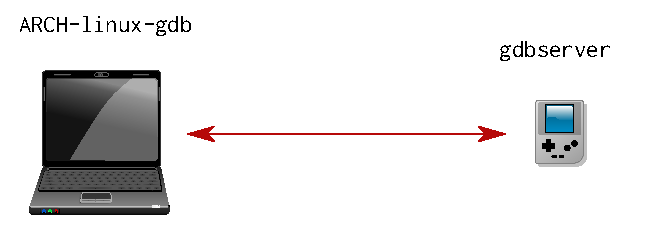
\includegraphics[width=0.5\textwidth]{common/gdb-vs-gdbserver.pdf}
  \end{center}


=== Remote debugging: architecture
  \begin{center}
    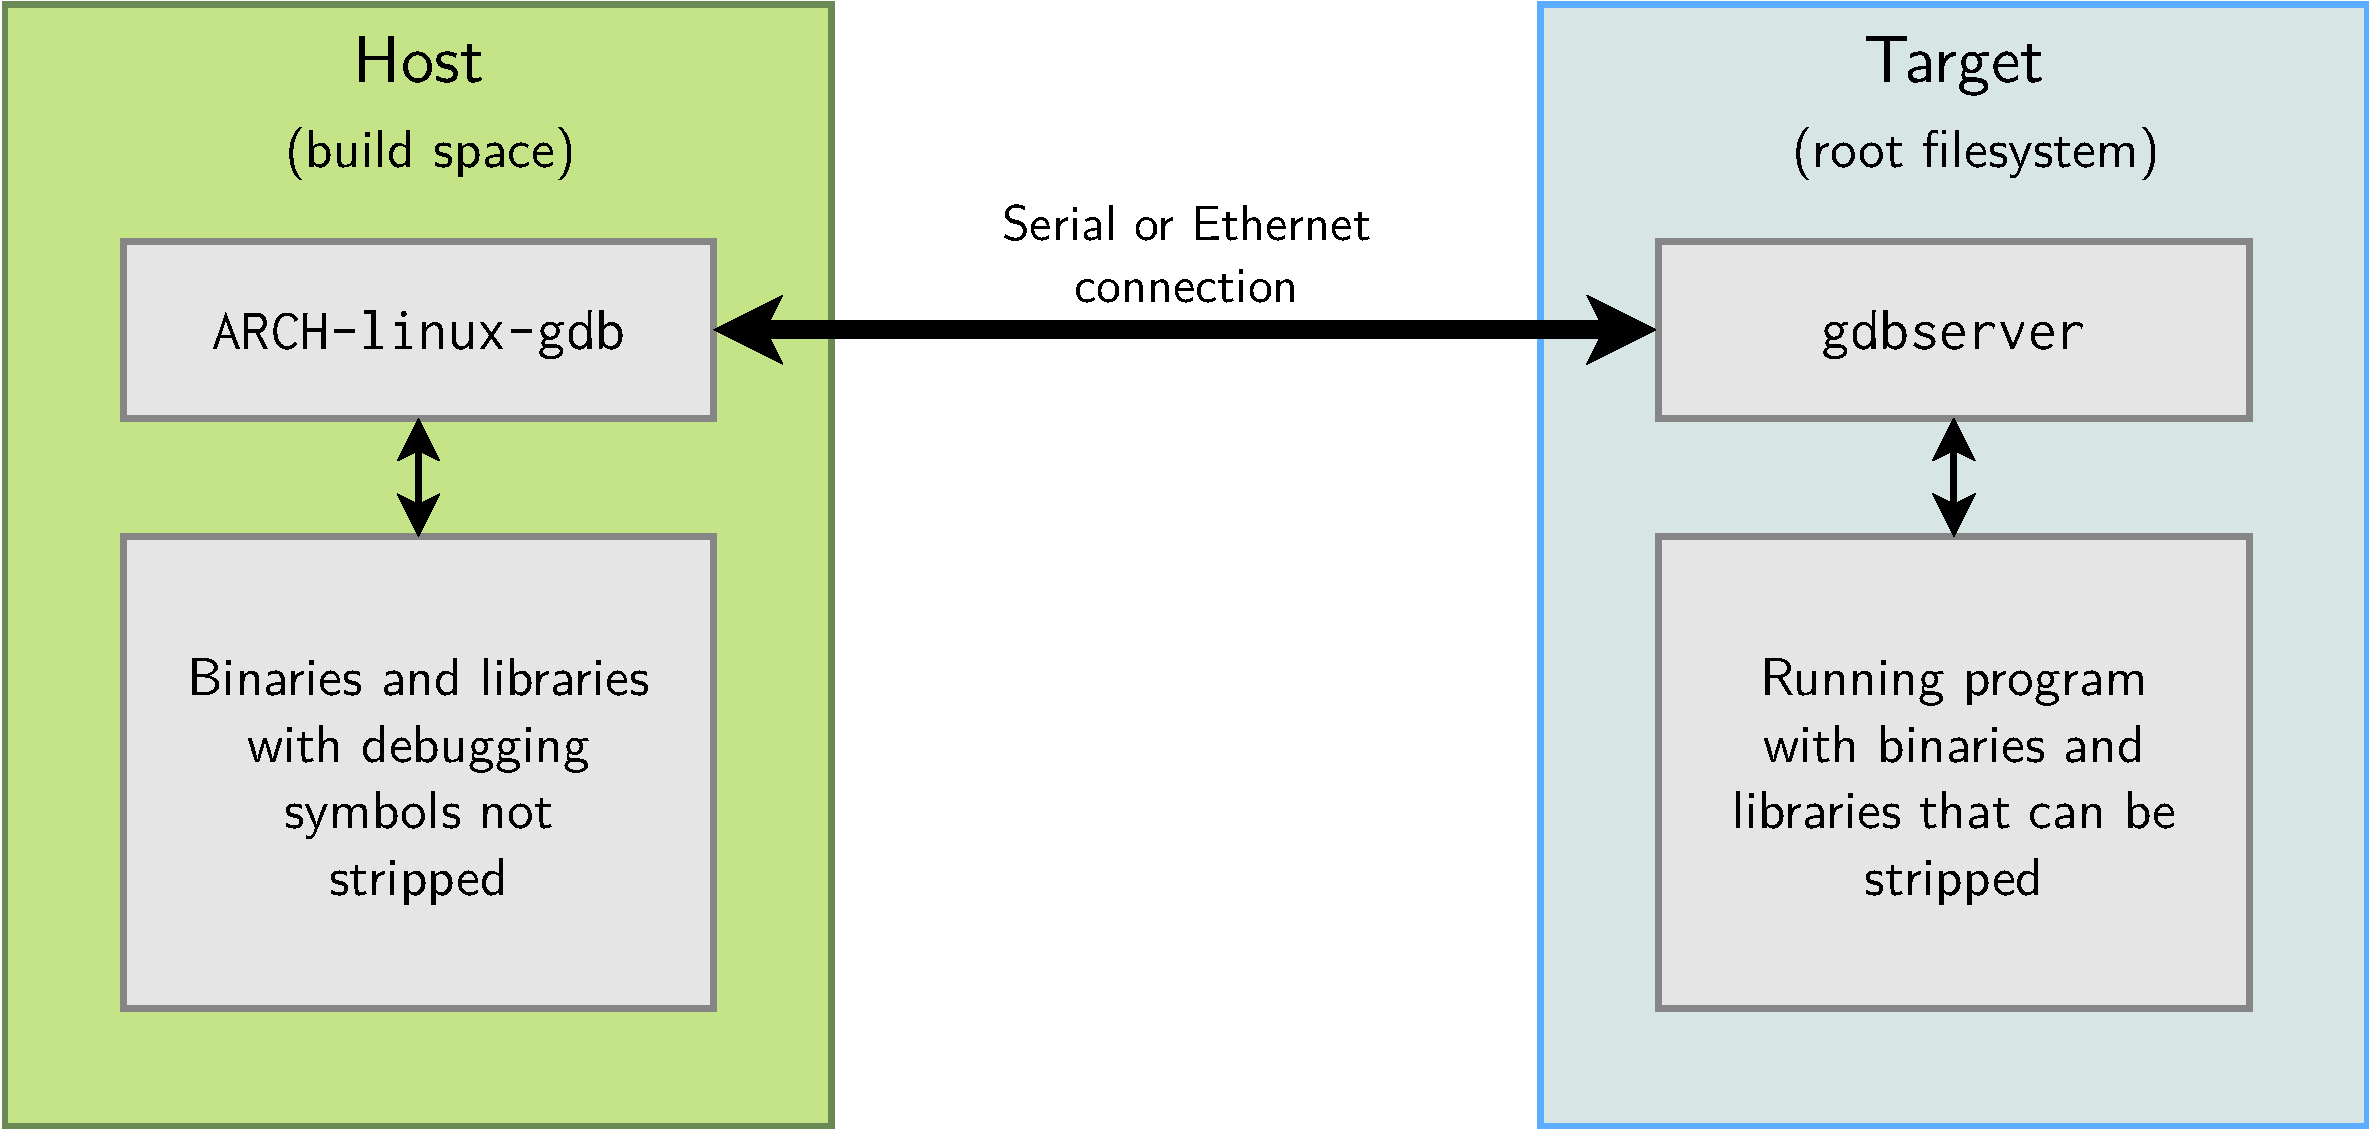
\includegraphics[width=\textwidth]{common/gdb-vs-gdbserver-architecture.pdf}
  \end{center}


=== Remote debugging: target setup
  \begin{itemize}
  \item On the target, run a program through `gdbserver`.\\
    Program execution will not start immediately.\\
    `gdbserver :<port> <executable> <args>`
    `gdbserver /dev/ttyS0 <executable> <args>`
  \item Otherwise, attach `gdbserver` to an already running program:\\
    `gdbserver --attach :<port> <pid>`
  \item You can also start gdbserver without passing any program to start or
  attach (and set the target program later, on client side):\\
    `gdbserver --multi :<port>`
  \end{itemize}


=== Remote debugging: host setup
  \begin{itemize}
  \item Then, on the host, start `ARCH-linux-gdb <executable>`,\\
    and use the following `gdb` commands:
    \begin{itemize}
    \item To tell `gdb` where shared libraries are:\\
      `gdb> set sysroot <library-path>` (typically path to build space without `lib/`)
    \item To connect to the target:\\
      `gdb> target remote <ip-addr>:<port>` (networking)\\
      `gdb> target remote /dev/ttyUSB0` (serial link)\\
      \begin{itemize}
        \item Make sure to replace `target remote` with `target
      extended-remote` if you have started gdbserver with the `--multi`
      option
      \end{itemize}
    \item If you did not set the program to debug on gdbserver commandline:\\
      `gdb> set remote exec-file <path_to_program_on_target>`
    \end{itemize}
  \end{itemize}


=== Coredumps for post mortem analysis
  \begin{itemize}
  \item It is sometime not possible to have a debugger attached when a
	  crash occurs
  \item Fortunately, Linux can generate a `core` file (a snapshot of
    the whole process memory at the moment of the crash), in the ELF
      format. gdb can use this `core` file to let us analyze the state
      of the crashed application
  \item On the target
    \begin{itemize}
    \item Use `ulimit -c unlimited` in the shell starting the
      application, to enable the generation of a `core` file
      when a crash occurs
    \item The output name and path for the coredump file can be modified using
	    `/proc/sys/kernel/core_pattern` (see #manpage("core", "5"))
		    \begin{itemize}
			    \item Example: `echo /tmp/mycore >
				    /proc/sys/kernel/core_pattern`
		    \end{itemize}
    \item Depending on the system configuration, the `core_pattern`
      file may be rewritten automatically by some software to handle core
        files or even disable core generation (eg: systemd)
    \end{itemize}
  \item On the host
    \begin{itemize}
    \item After the crash, transfer the `core` file from the target to
      the host, and run
      `ARCH-linux-gdb application-binary core-file`
    \end{itemize}
  \end{itemize}


=== minicoredumper
  \begin{itemize}
  \item Coredumps can be huge for complex applications
  \item minicoredumper is a userspace tool based on the standard core dump
    feature
    \begin{itemize}
    \item Based on the possibility to redirect the core dump output to a
      user space program via a pipe
    \end{itemize}
  \item Based on a JSON configuration file, it can:
    \begin{itemize}
    \item save only the relevant sections (stack, heap, selected ELF
      sections)
    \item compress the output file
    \item save additional information from `/proc`
    \end{itemize}
  \item \url{https://github.com/diamon/minicoredumper}
  \item ``Efficient and Practical Capturing of Crash Data on Embedded
    Systems''
    \begin{itemize}
      \item Presentation by minicoredumper author John Ogness
      \item Video: \url{https://www.youtube.com/watch?v=q2zmwrgLJGs}
      \item Slides:
        \href{https://elinux.org/images/8/81/Eoss2023_ogness_minicoredumper.pdf}
             {elinux.org/images/8/81/Eoss2023\_ogness\_minicoredumper.pdf}
    \end{itemize}
  \end{itemize}
\end{columns}